% Тип документа
\documentclass[a4paper,12pt]{extarticle}

% Шрифты, кодировки, символьные таблицы, переносы
\usepackage{cmap}
\usepackage[T2A]{fontenc}
\usepackage[utf8x]{inputenc}
\usepackage[russian]{babel}

% Это пакет -- хитрый пакет, он нужен но не нужен
\usepackage[mode=buildnew]{standalone}

\usepackage
	{
		% Дополнения Американского математического общества (AMS)
		amssymb,
		amsfonts,
		amsmath,
		amsthm,
		physics,
		% misccorr,
		% 
		% Графики и рисунки
		wrapfig,
		graphicx,
		subcaption,
		float,
		tikz,
		tikz-3dplot,
		caption,
		csvsimple,
		color,
		booktabs,
		pgfplots,
		pgfplotstable,
		geometry,
		% 
		% Таблицы, списки
		array,
		makecell,
		multirow,
		indentfirst,
		%
		% Интегралы и прочие обозначения
		ulem,
		esint,
		esdiff,
		% 
		% Колонтитулы
		fancyhdr,
	}  

\usepackage{xcolor}
\usepackage{hyperref}

 % Цвета для гиперссылок
\definecolor{linkcolor}{HTML}{000000} % цвет ссылок
\definecolor{urlcolor}{HTML}{799B03} % цвет гиперссылок
 
\hypersetup{pdfstartview=FitH,  linkcolor=linkcolor,urlcolor=urlcolor, colorlinks=true}
% Обводка текста в TikZ
\usepackage[outline]{contour}

% Увеличенный межстрочный интервал, французские пробелы
\linespread{1.3} 
\frenchspacing 

 
\usetikzlibrary
	{
		decorations.pathreplacing,
		decorations.pathmorphing,
		patterns,
		calc,
		scopes,
		arrows,
		fadings,
		through,
		shapes.misc,
		arrows.meta,
		3d,
		quotes,
		angles,
		babel
	}


\tikzset{
	force/.style=	{
		>=latex,
		draw=blue,
		fill=blue,
				 	}, 
	%				 	
	axis/.style=	{
		densely dashed,
		blue,
		line width=1pt,
		font=\small,
					},
	%
	th/.style=	{
		line width=1pt},
	%
	acceleration/.style={
		>=open triangle 60,
		draw=magenta,
		fill=magenta,
					},
	%
	inforce/.style=	{
		force,
		double equal sign distance=2pt,
					},
	%
	interface/.style={
		pattern = north east lines, 
		draw    = none, 
		pattern color=gray!60,
					},
	cross/.style=	{
		cross out, 
		draw=black, 
		minimum size=2*(#1-\pgflinewidth), 
		inner sep=0pt, outer sep=0pt,
					},
	%
	cargo/.style=	{
		rectangle, 
		fill=black!70, 
		inner sep=2.5mm,
					},
	%
	caption/.style= {
		midway,
		fill=white!20, 
		opacity=0.9
					},
	%
	}

\newenvironment{tikzpict}
    {
	    \begin{figure}[htbp]
		\centering
		\begin{tikzpicture}
    }
    { 
		\end{tikzpicture}
		% \caption{caption}
		% \label{fig:label}
		\end{figure}
    }


\newcommand{\vbLabel}[3]{\draw ($(#1,#2)+(0,5pt)$) -- ($(#1,#2)-(0,5pt)$) node[below]{#3}}
\newcommand{\vaLabel}[3]{\draw ($(#1,#2)+(0,5pt)$) node[above]{#3} -- ($(#1,#2)-(0,5pt)$) }

\newcommand{\hrLabel}[3]{\draw ($(#1,#2)+(5pt,0)$) -- ($(#1,#2)-(5pt,0)$) node[right, xshift=1em]{#3}}
\newcommand{\hlLabel}[3]{\draw ($(#1,#2)+(5pt,0)$) node[left, xshift=-1em]{#3} -- ($(#1,#2)-(5pt,0)$) }



\newcommand\zi{^{\,*}_i}
\newcommand\sumn{\sum_{i=1}^{N}}

\tikzset{
	coordsys/.style={scale=1.8,x={(1.1cm,-0cm)},y={(0.5cm,1cm)}, z={(0cm,0.8cm)}},
	coordsys/.style={scale=1.5,x={(0cm,0cm)},y={(1cm,0cm)}, z={(0cm,1cm)}}, 
	coordsys/.style={scale=1.5,x={(1cm,0cm)},y={(0cm,1cm)}, z={(0cm,0cm)}}, 
}

\usepgfplotslibrary{units}


% Draw line annotation
% Input:
%   #1 Line offset (optional)
%   #2 Line angle
%   #3 Line length
%   #5 Line label
% Example:
%   \lineann[1]{30}{2}{$L_1$}

\newcommand{\lineann}[4][0.5]{%
    \begin{scope}[rotate=#2, blue,inner sep=2pt, ]
        \draw[dashed, blue!40] (0,0) -- +(0,#1)
            node [coordinate, near end] (a) {};
        \draw[dashed, blue!40] (#3,0) -- +(0,#1)
            node [coordinate, near end] (b) {};
        \draw[|<->|] (a) -- node[fill=white, scale=0.8] {#4} (b);
    \end{scope}
}

\newcommand{\lineannn}[4][0.5]{%
    \begin{scope}[rotate=#2, blue,inner sep=2pt, ]
        \draw[dashed, blue!40] (0,0) -- +(0,#1)
            node [coordinate, near end] (a) {};
        \draw[dashed, blue!40] (#3,0) -- +(0,#1)
            node [coordinate, near end] (b) {};
        % \draw[color=white, color=blue] (a) -- node[fill=white, scale=0.8] {#4} (b);
        \draw[->|] (a)++(-0.3,0) -- (a);
        \draw[->|] (b)++(0.3,0) coordinate (xx) -- (b);
        \draw (xx) node[fill=white, scale=0.8, right] {#4};
    \end{scope}
}

% Круговая стрелка относительно центра (дуга из центра)
\tikzset{
  pics/carc/.style args={#1:#2:#3}{
    code={
      \draw[pic actions] (#1:#3) arc(#1:#2:#3);
    }
  },
  dash/.style={
  	dash pattern=on 5mm off 5mm
  }
}

% Среднее <#1>
\newcommand{\mean}[1]{\langle#1\rangle}

\pgfplotsset{
    % most recent feature set of pgfplots
    compat=newest,
}

% const прямым шрифтом
\newcommand\ct[1]{\text{\rmfamily\upshape #1}}
\newcommand*{\const}{\ct{const}}


\usepackage[europeanresistors,americaninductors]{circuitikz}

% Style to select only points from #1 to #2 (inclusive)
\pgfplotsset{select/.style 2 args={
    x filter/.code={
        \ifnum\coordindex<#1\def\pgfmathresult{}\fi
        \ifnum\coordindex>#2\def\pgfmathresult{}\fi
    }
}}


\usepackage{array}
\usepackage{pstool}


%%%%%%%%%%%%%%%%%%%%%%%%%%%%%%%%%%%%%%%%%%%%%%%%%
\makeatletter
\newif\if@gather@prefix 
\preto\place@tag@gather{% 
  \if@gather@prefix\iftagsleft@ 
    \kern-\gdisplaywidth@ 
    \rlap{\gather@prefix}% 
    \kern\gdisplaywidth@ 
  \fi\fi 
} 
\appto\place@tag@gather{% 
  \if@gather@prefix\iftagsleft@\else 
    \kern-\displaywidth 
    \rlap{\gather@prefix}% 
    \kern\displaywidth 
  \fi\fi 
  \global\@gather@prefixfalse 
} 
\preto\place@tag{% 
  \if@gather@prefix\iftagsleft@ 
    \kern-\gdisplaywidth@ 
    \rlap{\gather@prefix}% 
    \kern\displaywidth@ 
  \fi\fi 
} 
\appto\place@tag{% 
  \if@gather@prefix\iftagsleft@\else 
    \kern-\displaywidth 
    \rlap{\gather@prefix}% 
    \kern\displaywidth 
  \fi\fi 
  \global\@gather@prefixfalse 
} 
\newcommand*{\beforetext}[1]{% 
  \ifmeasuring@\else
  \gdef\gather@prefix{#1}% 
  \global\@gather@prefixtrue 
  \fi
} 
\makeatother
%%%%%%%%%%%%%%%%%%%%%%%%%%%%%%%%%%%%%%%%%%%%%%%%%

\geometry		
	{
		left			=	2cm,
		right 			=	2cm,
		top 			=	3cm,
		bottom 			=	3cm,
		bindingoffset	=	0cm
	}

%%%%%%%%%%%%%%%%%%%%%%%%%%%%%%%%%%%%%%%%%%%%%%%%%%%%%%%%%%%%%%%%%%%%%%%%%%%%%%%



	%применим колонтитул к стилю страницы
\pagestyle{fancy} 
	%очистим "шапку" страницы
\fancyhead{} 
	%слева сверху на четных и справа на нечетных
\fancyhead[R]{\labauthors} 
	%справа сверху на четных и слева на нечетных
\fancyhead[L]{Отчёт по лабораторной работе №\labnumber} 
	%очистим "подвал" страницы
\fancyfoot{} 
	% номер страницы в нижнем колинтуле в центре
\fancyfoot[C]{\thepage} 

%%%%%%%%%%%%%%%%%%%%%%%%%%%%%%%%%%%%%%%%%%%%%%%%%%%%%%%%%%%%%%%%%%%%%%%%%%%%%%%

\renewcommand{\contentsname}{Оглавление}

\usepackage{tocloft}
% \renewcommand{\cftpartleader}{\cftdotfill{\cftdotsep}} % for parts
% \renewcommand{\cftsectiondotsep}{\cftdotsep}% Chapters should use dots in ToC
\renewcommand{\cftsecleader}{\cftdotfill{\cftdotsep}}
%\renewcommand{\cftsecleader}{\cftdotfill{\cftdotsep}} % for sections, if you really want! (It is default in report and book class (So you may not need it).
% ---------
% \newcommand{\cftchapaftersnum}{.}%
% \usepackage{titlesec}
% \titlelabel{\thetitle.\quad}
\usepackage{secdot}
\sectiondot{subsection}
\usepackage{pgfplots,pgfplotstable,booktabs,colortbl}
\pgfplotsset{compat=newest}
\usepackage{physics}
\usepackage{mathtools}
\mathtoolsset{showonlyrefs=true}
\newcommand\Smat{\hat { \mathbf { S } }}

\newcommand*\dotvec[1][1,1]{\crossproducttemp#1\relax}
\def\crossproducttemp#1,#2\relax{{\qty[\vec{#1}\times\vec{#2}\,]}}

\newcommand*\prodvec[1][1,1]{\crossproducttempa#1\relax}
\def\crossproducttempa#1,#2\relax{{\qty[{#1}\times{#2}\,]}}
\renewcommand{\vec}{\mathbf} % for parts

\def\Rdim{\,\frac{\text{м}^3}{\text{А} \cdot \text{с}}}
\renewcommand{\phi}{\varphi}
\renewcommand{\labelenumii}{\theenumii)} 
% \newcommand{\mean}[1]{\langle#1\rangle}
% 
% \mathtoolsset{showonlyrefs=true}
% \newcommand\Smat{\hat { \mathbf { S } }}
\let\tempint\int
\renewcommand{\int}{\tempint\limits}
\DeclareMathOperator{\Div}{div}
\DeclareMathOperator{\Rot}{rot}
\DeclareMathOperator{\Grad}{grad}
\renewcommand{\phi}{\varphi}

\begin{document}

\def\labauthors{Виноградов И.Д., Шиков А.П.}
\def\labgroup{430}
\def\labnumber{2}
\def\labtheme{Движение носителей заряда в электрических и магнитных полях. Эффект Холла}
\begin{titlepage}

\begin{center}

{\small\textsc{Нижегородский государственный университет имени Н.\,И. Лобачевского}}
\vskip 1pt \hrule \vskip 3pt
{\small\textsc{Радиофизический факультет. Кафедра Радиотехники.}}

\vfill

{\Large Отчет по лабораторной работе №\labnumber\vskip 12pt\bfseries \labtheme}
	
\end{center}

\vfill
	
\begin{flushright}
	{Выполнили студенты \labgroup\ группы\\ \labauthors}%\vskip 12pt Принял:\\ Менсов С.\,Н.}
\end{flushright}
	
\vfill
	
\begin{center}
	Нижний Новгород, \the\year
\end{center}

\end{titlepage}



\newpage

\section*{Введение}
	Особенности движения носителей заряда в электрических и магнитных
полях определяют специфику функционирования подавляющего большинства
приборов современной микроэлектроники. Данное описание содержит краткое
изложение элементарных основ теории явлений переноса носителей заряда в 
однородном полупроводниковом материале. При этом речь пойдет как о движении
в электрических полях различной напряженности, однородно и неоднородно
распределенных в пространстве, так и о движении в скрещенных электрических
и магнитных полях, т.е. в условиях проявления эффекта Холла.
Для работы любой радиолинии необходимо, чтобы ток возбуждения антенны на её передающем конце отображал передаваемый сигнал, т.е. необходимо каким-то образом «записать» его на токе высокой частоты.
\section*{Теоретическая часть}

\section{Элементарная теория эффекта Холла}
Анализ транспорта носителей в полупроводниковых структурах, требует знания
концентрации носителей заряда и их подвижности в материале. Эти характеристики являются важными физическими величинами,
определяющими многие свойства полупроводников, например, электропроводность, теплопроводность, термо-ЭДС и др.

Концентрацию и подвижность в отдельности можно определить, зная соотношение между ними. В данной работе это соотношение
устанавливается экспериментально при помощи эффекта Холла.

Эффект Холла представляет собой поперечный гальваномагнитный эффект, суть которого заключается в следующем: если
поместить полупроводниковую пластину во внешнее магнитное поле $\vec B$ (рис. \ref{fig:8}) и пропустить вдоль нее ток,
то вследствие смещения движущихся зарядов к одной из граней пластины возникает поперечная разность потенциалов,
называемая \textit{ЭДС Холла}. При этом (см. рис. \ref{fig:8}.б, \ref{fig:8}.в), носители различных знаков смещаются к
одной и той же боковой грани полупроводника, поэтому с изменением типа электропроводности меняется и знак ЭДС.

С помощью эффекта Холла можно экспериментально определить тип носителей, концентрацию и подвижность в данном
полупроводниковом образце. Другим важным практическим приложением этого эффекта являются измерения силы тока и мощности
в цепях постоянного и переменного тока  (вплоть до очень высоких частот), напряженности постоянных и переменных
магнитных полей, преобразование сигналов, анализ спектров и т.д.

\begin{figure}[h!]
\begin{minipage}[h]{0.329\linewidth}
		\centering
	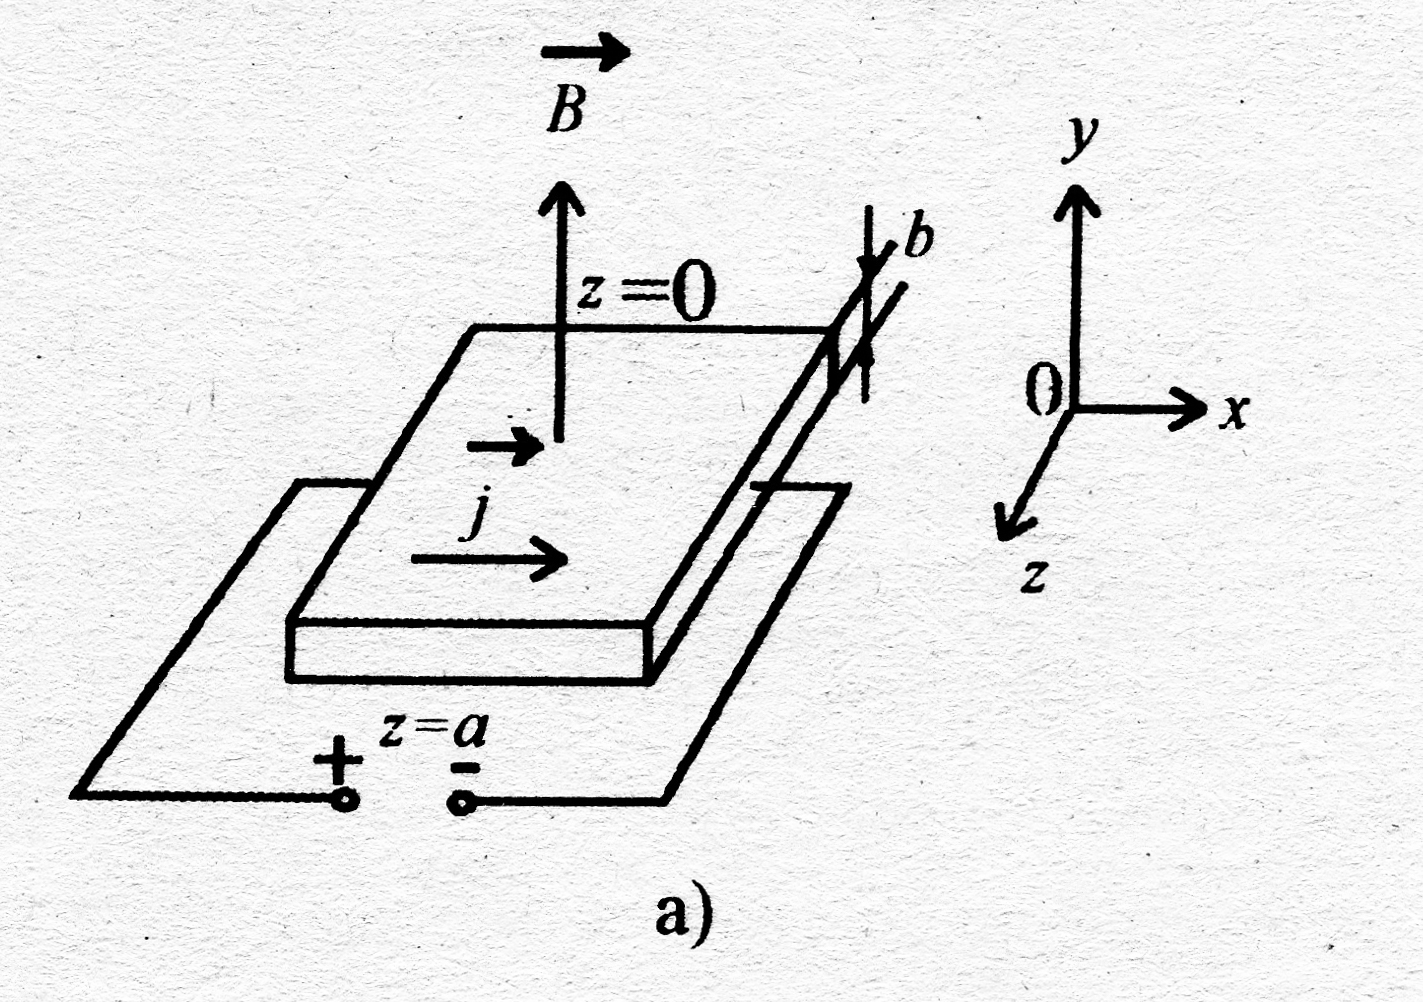
\includegraphics[width=\linewidth]{fig/21a}
\end{minipage}
\begin{minipage}[h]{0.329\linewidth}
		\centering
	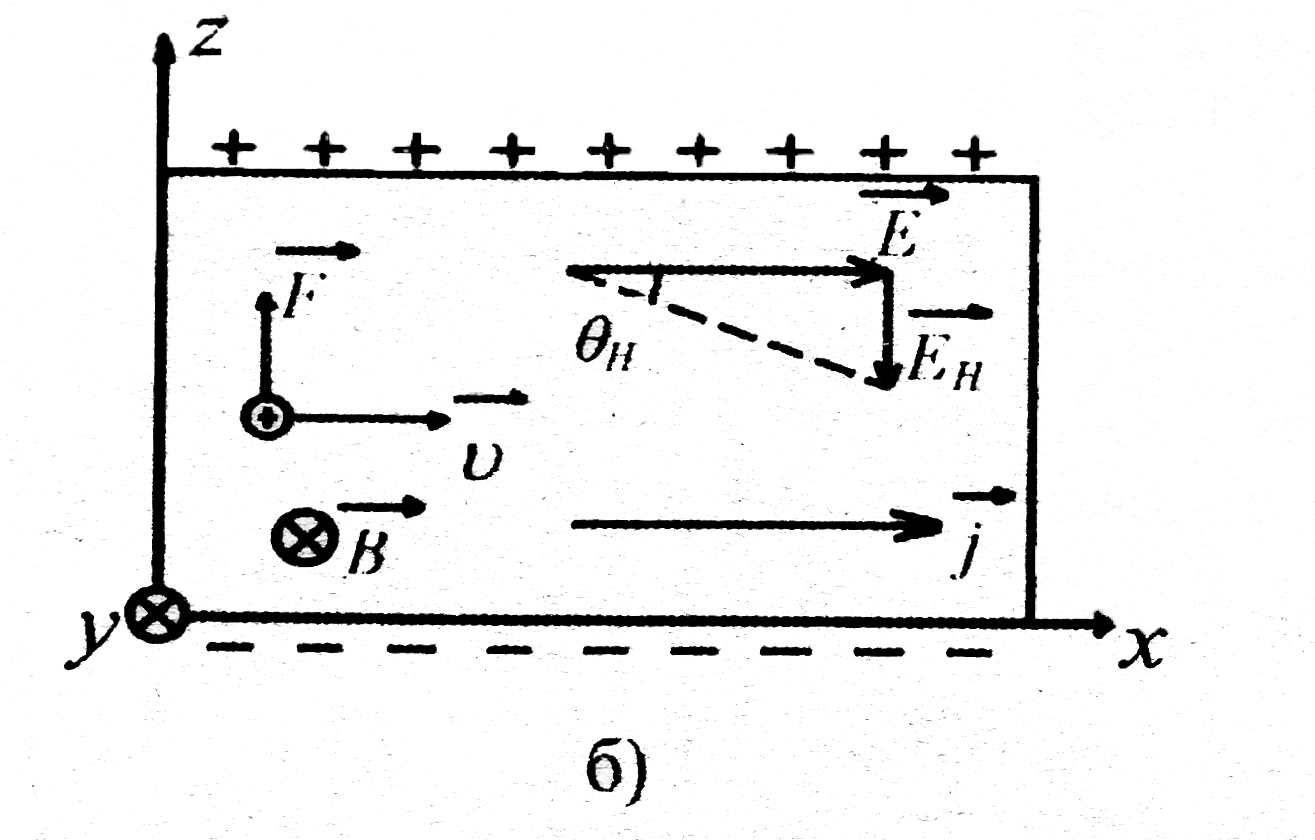
\includegraphics[width=\linewidth]{fig/21b}
\end{minipage}
\begin{minipage}[h]{0.329\linewidth}
		\centering
	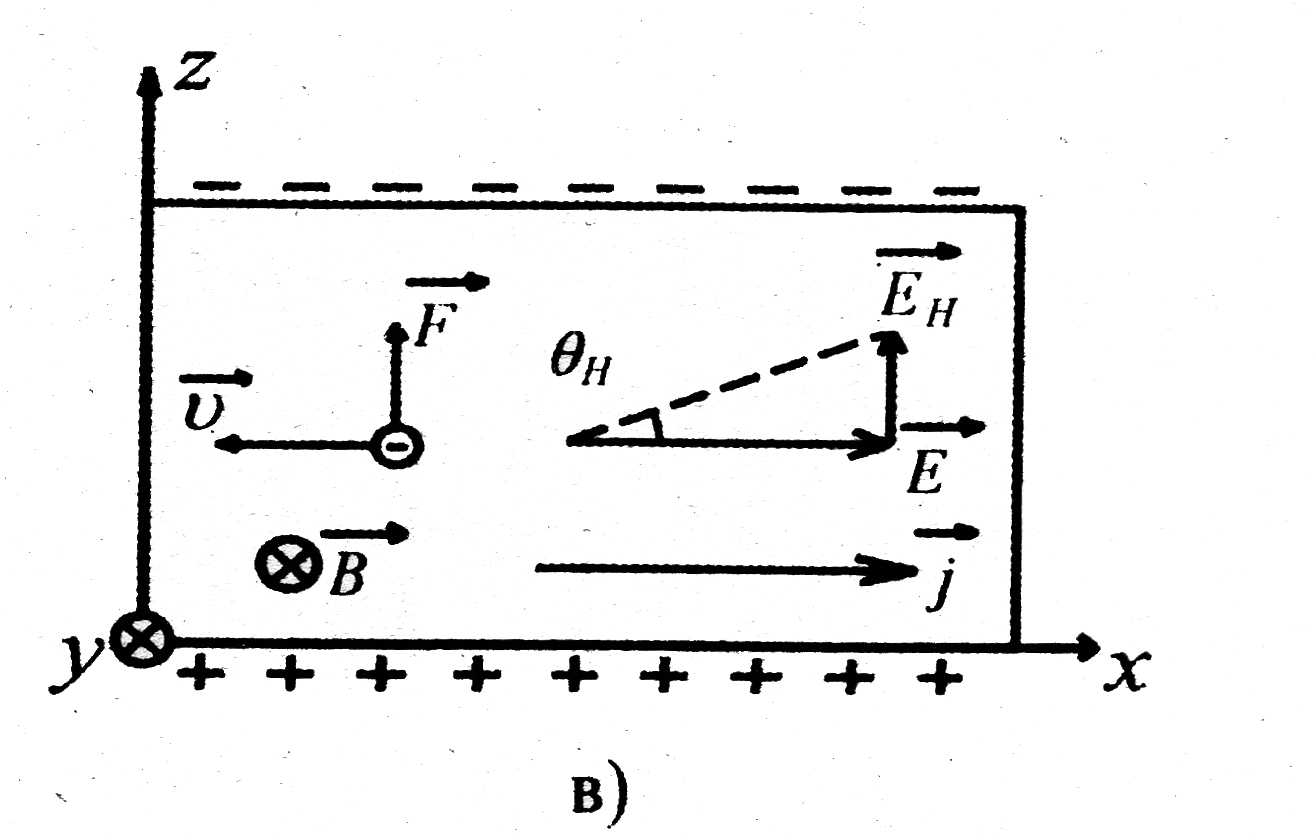
\includegraphics[width=\linewidth]{fig/21c}
\end{minipage}
	\caption{Возникновение ЭДС Холла: схема эксперимента (а); смещение носителей заряда в дырочном (б) и электронном (в) полупроводниках, соответственно}
	\label{fig:8}
\end{figure}

Разберем эффект Холла более подробно. На рис. \ref{fig:8}.а показан полупроводник, две плоскости которого подключены
через омические (т.е. невыпрямляющие) контакты к внешней батарее. Обозначим $\vec j$ плотность тока в направлении Ox.
Магнитное поле $\vec B$ приложено в направлении Oy. Рассмотрим электрон, двигающийся в отрицательном направлении оси Ox
со средней скоростью $\vec V$. На движущийся в магнитном поле электрон действует магнитная составляющая силы Лоренца:
$$\vec F = -e [\vec v, \vec B].$$
В результате действия этой силы траектория электрона будет искривляться  в направлении оси z, и, поскольку в этом
направлении ток протекать не может, электроны будут накапливаться на боковой поверхности ($z=\pm a$, см. рис.
\ref{fig:8}) до тех пор, пока не установится электрическое поле $\vec E_H$, достаточное для создания силы. равной
магнитной составляющей силы Лоренца, но направленной противоположно. Приравнивая эти силы, получим: 
\begin{equation}
\label{eq:2.1}
	\vec E_H=[\vec v, \vec B]
\end{equation}

Воспользуемся законом Ома в дифференциальной форме:
\begin{equation}
\label{eq:2.2}
	\vec j = \sigma \vec E,
\end{equation}
где $\sigma = e \cdot n \cdot \mu_n$ - удельная проводимость образца, $\mu_n = \frac{v}{E}$ - подвижность носителей. Соотношение \eqref{eq:2.2} перепишем в следующем виде:
\begin{equation}
\label{eq:2.3}
	\vec j = e \cdot n \cdot \mu_n \cdot \vec E = -e \cdot n \cdot \vec v
\end{equation}

Исключая $v$ из соотношения \eqref{eq:2.1}, получим:
\begin{equation}
\label{eq:2.4}
	\vec E_H = -\frac{1}{en} [\vec j, \vec B]=R[\vec j, \vec B]
\end{equation}

Учитывая, что полный ток через образец $I=jab$, а поперечная ЭДС $U_H=E_Ha$, получим соотношение, связывающее ЭДС Холла с величиной электрического тока:
\begin{equation}
\label{eq:2.5}
	U_H=R \cdot \frac{I\cdot B}{b}
\end{equation}

Величина R называется \textit{постоянной Холла} и определяется как

\begin{equation}
\label{eq:2.6}
	R=-\frac{1}{e\cdot n}
\end{equation}

Поперечную ЭДС $U_H$, ток I, напряженность магнитного поля B (для немагнитных образцов) и толщину b полупроводникового
образца можно измерить. Это позволяет найти численное значение постоянной Холла.

В действительности, произведенный элементарный вывод коэффициента Холла \eqref{eq:2.6} неточен: в нем не учтена разница
между мгновенной скоростью электронов, входящей в выражение магнитной составляющей силы Лоренца, и дрейфовой скоростью,
которую электрон приобретает под действием электрического поля. Кроме того, не учитывается распределение электронов по
скоростям и механизмы рассеяния носителей. Формула \eqref{eq:2.6} оказывается справедливой только для металлов и
вырожденных полупроводников (вырожденным называется полупроводник с очень высокой, порядка $10^{19}$ атом/$\text{см}^3$,
концентрацией примеси). Более строгий анализ дает для невырожденных полупроводников значение R, которое отличается от
выражения \eqref{eq:2.6} множителем А. Если учитывать рассеяние носителей только на кристаллической решетке
(взаимодействие с фононами), то $A=\frac{3\pi}{8}$. В общем виде постоянная Холла может быть записана как:
\begin{gather}
	R=-\frac{A}{n\cdot e} \text{(для полупроводника n-типа)} \notag \\
	R=\frac{A}{p\cdot e} \text{(для полупроводника p-типа)}
\label{eq:2.7}
\end{gather}
где множитель А может принимать значения от 1 до 1.7. Знак минус в формуле \eqref{eq:2.7} демонстрирует, что ЭДС Холла
для электронного полупроводника имеет полярность, противоположную полярности для дырочного полупроводника.

Знание электропроводности и постоянной Холла позволяет найти как концентрацию носителей, так и их подвижность.

Обозначим через холловский угол $\theta_H$ малый угол, который образует с осью х вектор напряженности суммарного электрического поля (см. рис. \ref{fig:8}):
\begin{equation}
\label{eq:2.8}
	\theta_H \cong \tg{\theta_H}=\frac{E_H}{E}
\end{equation}

Из \ref{eq:2.8} с учетом \ref{eq:2.2} и \ref{eq:2.4} получим:
\begin{equation}
\label{eq:2.9}
	\theta_H = \mu_{nH} \cdot B
\end{equation}
где $\theta_H$-холловский угол в проводнике n-типа, а $\mu_{nH}$ - так называемая \textit{холловская подвижность} электронов (индекс H указывает на метод определения подвижности). Численное значение холловской подвижности может расходиться с величиной подвижности, определенной другими методами (например, прямым способом, основанным на измерении времени распространения носителей тока по полупроводнику на определенное расстояние с известным ускоряющим полем). Последняя называется дрейфовой подвижностью. Дрейфовую подвижность можно определить из выражения \ref{eq:2.4}, если, используя выражение \ref{eq:2.7}, преобразовать его к виду:
\begin{equation}
\label{eq:2.10}
	\vec E_H = -\frac{A}{en}\cdot[\vec j, \vec B]=-A\cdot \mu_{nd} \cdot [\vec E,\vec B],
\end{equation}
где индекс d при $\mu_{nd}$ указывает, что это дрейфовая подвижность электронов.

Из выражений \eqref{eq:2.8}-\eqref{eq:2.10} следует, что для электронов $\mu_{nH}=A\cdot \mu_{nd}$, а для дырок $\mu_{pH}=A\cdot \mu_{pd}$. Используя выражения \eqref{eq:2.2} и \eqref{eq:2.7}, получим:
\begin{equation}
\label{eq:2.11}
	\mu_{(n,p)H}=R\cdot \sigma.
\end{equation}

Приведенные выше выражения относились к полупроводникам, у которых концентрация неосновных носителей пренебрежимо мала
по сравнению с концентрацией основных (униполярная проводимость). 

\newpage
\section*{Эксперимент}
\textbf{Оборудование}
\begin{enumerate}
\item Источник питания образца GPS-3030D.
\item Мультиметр APPA201N в режиме измерения постоянного напряжения на пределе 200 мВ.
\item Согласующий модуль
\item Исследуемый образец ($l = 22 \text{ мм},w = 1.9 \text{ мм}, d = 0.33 \text{ мм}$)
\item Электромагнит в виде катушки с обмоткой из медного провода
\item Источник питания электромагнита GPS-3030D.
\end{enumerate}

\subsection*{Схема лабораторной установки}

\begin{figure}[h!]
	\centering
	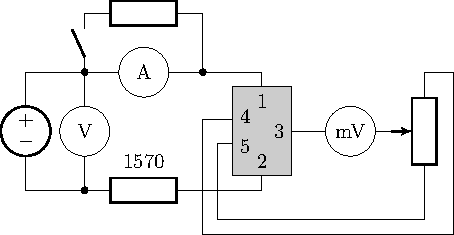
\includegraphics[scale=1.5]{ris/chem.pdf}
	\caption{Принципиальная схема включения (использовалось только направление $1\to2$)}
	\label{fig:figure2}
\end{figure}

Напряжение с источника питания GPS-3030D, работающего в режиме стабилизации напряжения, подаётся на образец через
ограничительный резистор R1. Измерение тока образца производится стрелочным миллиамперметром, находящимся на передней
панели согласующего модуля. Переключение пределов измерения миллиамперметра (10 мА – 3 мА) позволяет увеличить точность
измерения тока образца. Сопротивление миллиамперметра при работе на пределе «3 мА» – 171 Ом, на пределе «10 мА» – 51 Ом.
Для изменения направления тока через образец служит переключатель «Направление тока», имеющий среднее положение, в
котором образец отключён от источника питания.
Для измерения ЭДС Холла используется мультиметр в режиме измерения постоянного напряжения на пределе 200 мВ. 

Один из выводов мультиметра подсоединяется к контакту 3 образца, другой – к резистору R2 <<Балансировка>>.


\section*{Практическая часть}
\subsection*{Измерение ВАХ образца и паразитного напряжения на контактах}

\begin{figure}[h!]
	\centering
	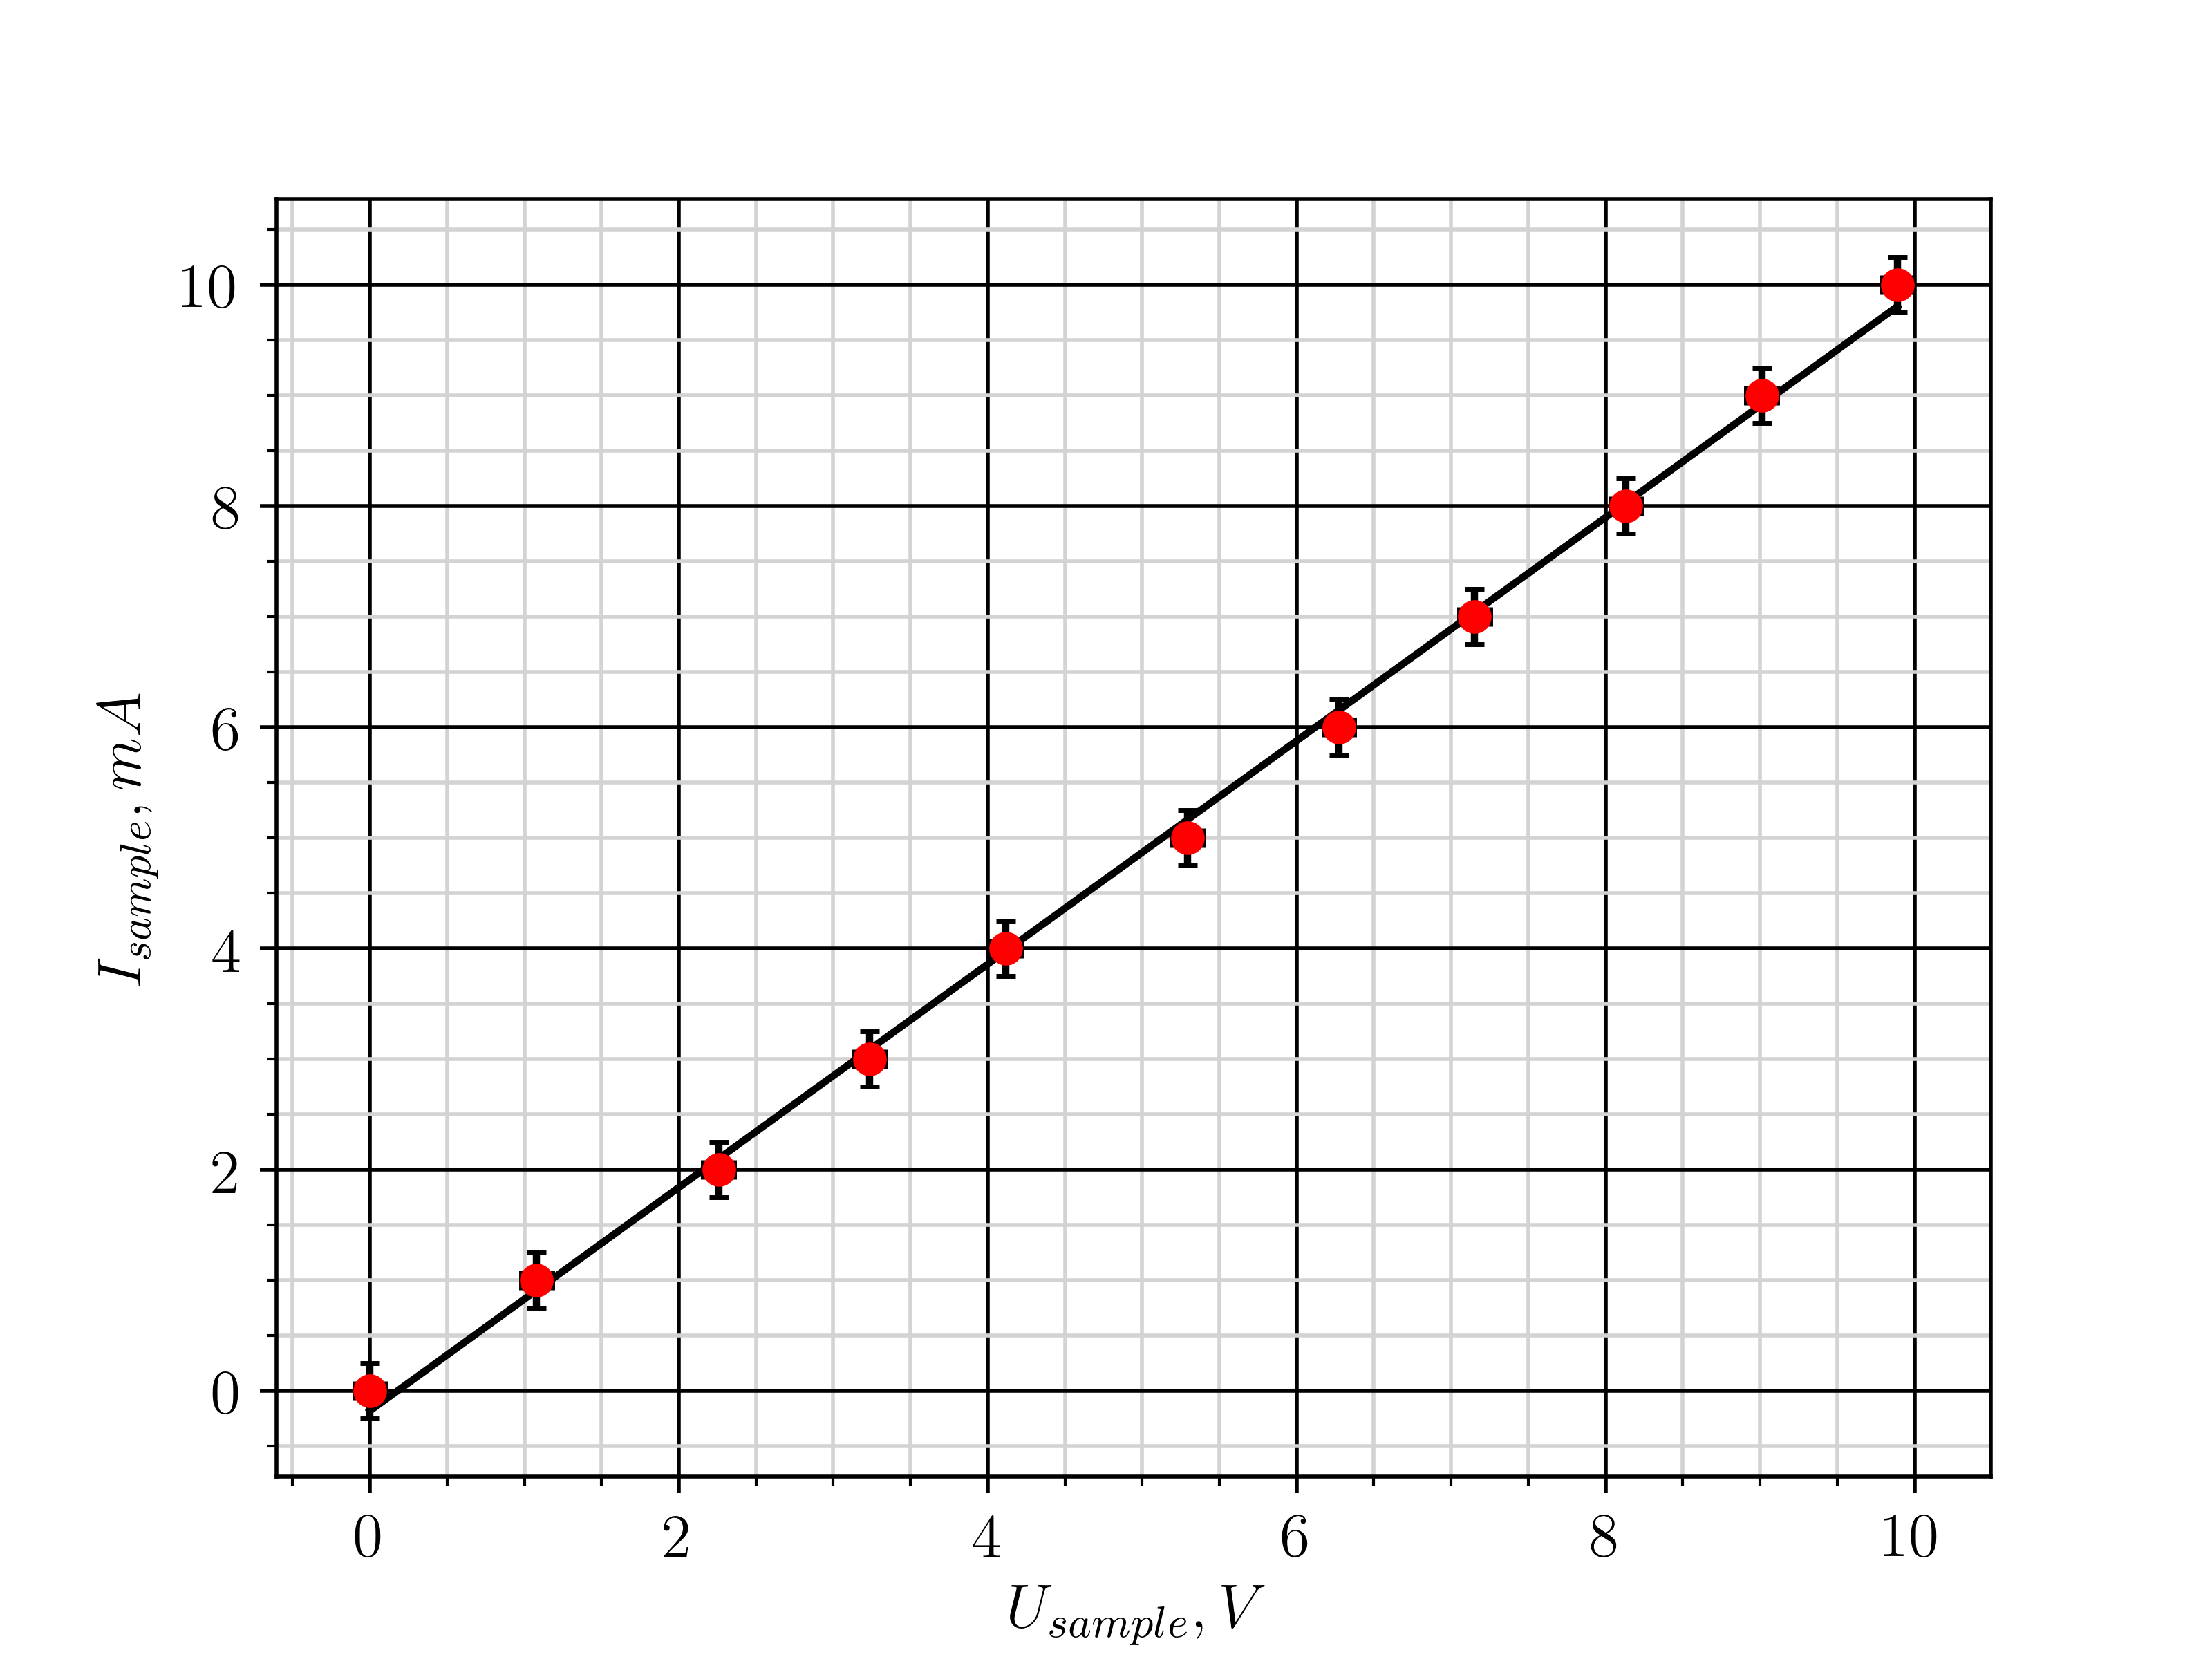
\includegraphics[width = .9\linewidth]{graphs/voltamp.png}
	\caption{ВАХ образца}
	\label{fig:5.2}
\end{figure}

На рис. \ref{fig:5.2} изображена ВАХ образца (Погрешность тока $\Delta I_{sample} = I_{\max}\cdot 2.5\% = \pm 0.25
\text{ мА}$, погрешность напряжения $\Delta U = \pm 0.1 V$). Учитывая, что снимаемое напряжение - это напряжение на всей цепи, включая
образец, то напряжение на образце было рассчитано из закона Ома:
\begin{equation}
		U_{gen} = U_{sample} + I \cdot (R_1+51)
\end{equation}
\begin{equation}
	U_{sample} = U_{gen} - I \cdot (1621)
\end{equation}
По переменным напряжения и тока построена линейная регрессия,
показывающая, что данные хорошо апроксимируются прямой.


Исходя из полученной линейной зависимости (наклон прямой), учитывая погрешность измерительных приборов, найдено сопротивление образца , и
полное сопротивление цепи. Согласно схеме установки, в цепь последовательно включено сопротивление $R_1=1570$ Ом +
сопротивление амперметра, отсюда
\begin{equation}
	R_{sample}=1010 \pm25 \text{ Ом} \quad
	R_\text{цепи}=2630 \pm25 \text{ Ом}, \quad
\end{equation}
Исходя из ранее известных размеров образца: длины $l=2.2\cdot 10^{-2}$ м, ширины  $w=1.9\cdot 10^{-3}$ м и толщины $d=3.3\cdot 10^{-4} $ м, получены удельные сопротивление и проводимость материала образца:
\begin{equation}
	\rho=\frac{R_{sample}\cdot S}{l}=\frac{R_{sample}\cdot w \cdot d}{l}=
	0.029\pm 7 \cdot 10^{-4} \text{ Ом$\cdot$м}
\end{equation}

\begin{equation}
	\sigma=\frac{1}{\rho}=34.1\pm0.1 \text{ Ом$^{-1}\cdot$м$^{-1}$}
\end{equation}

\begin{figure}[h!]
	\centering
		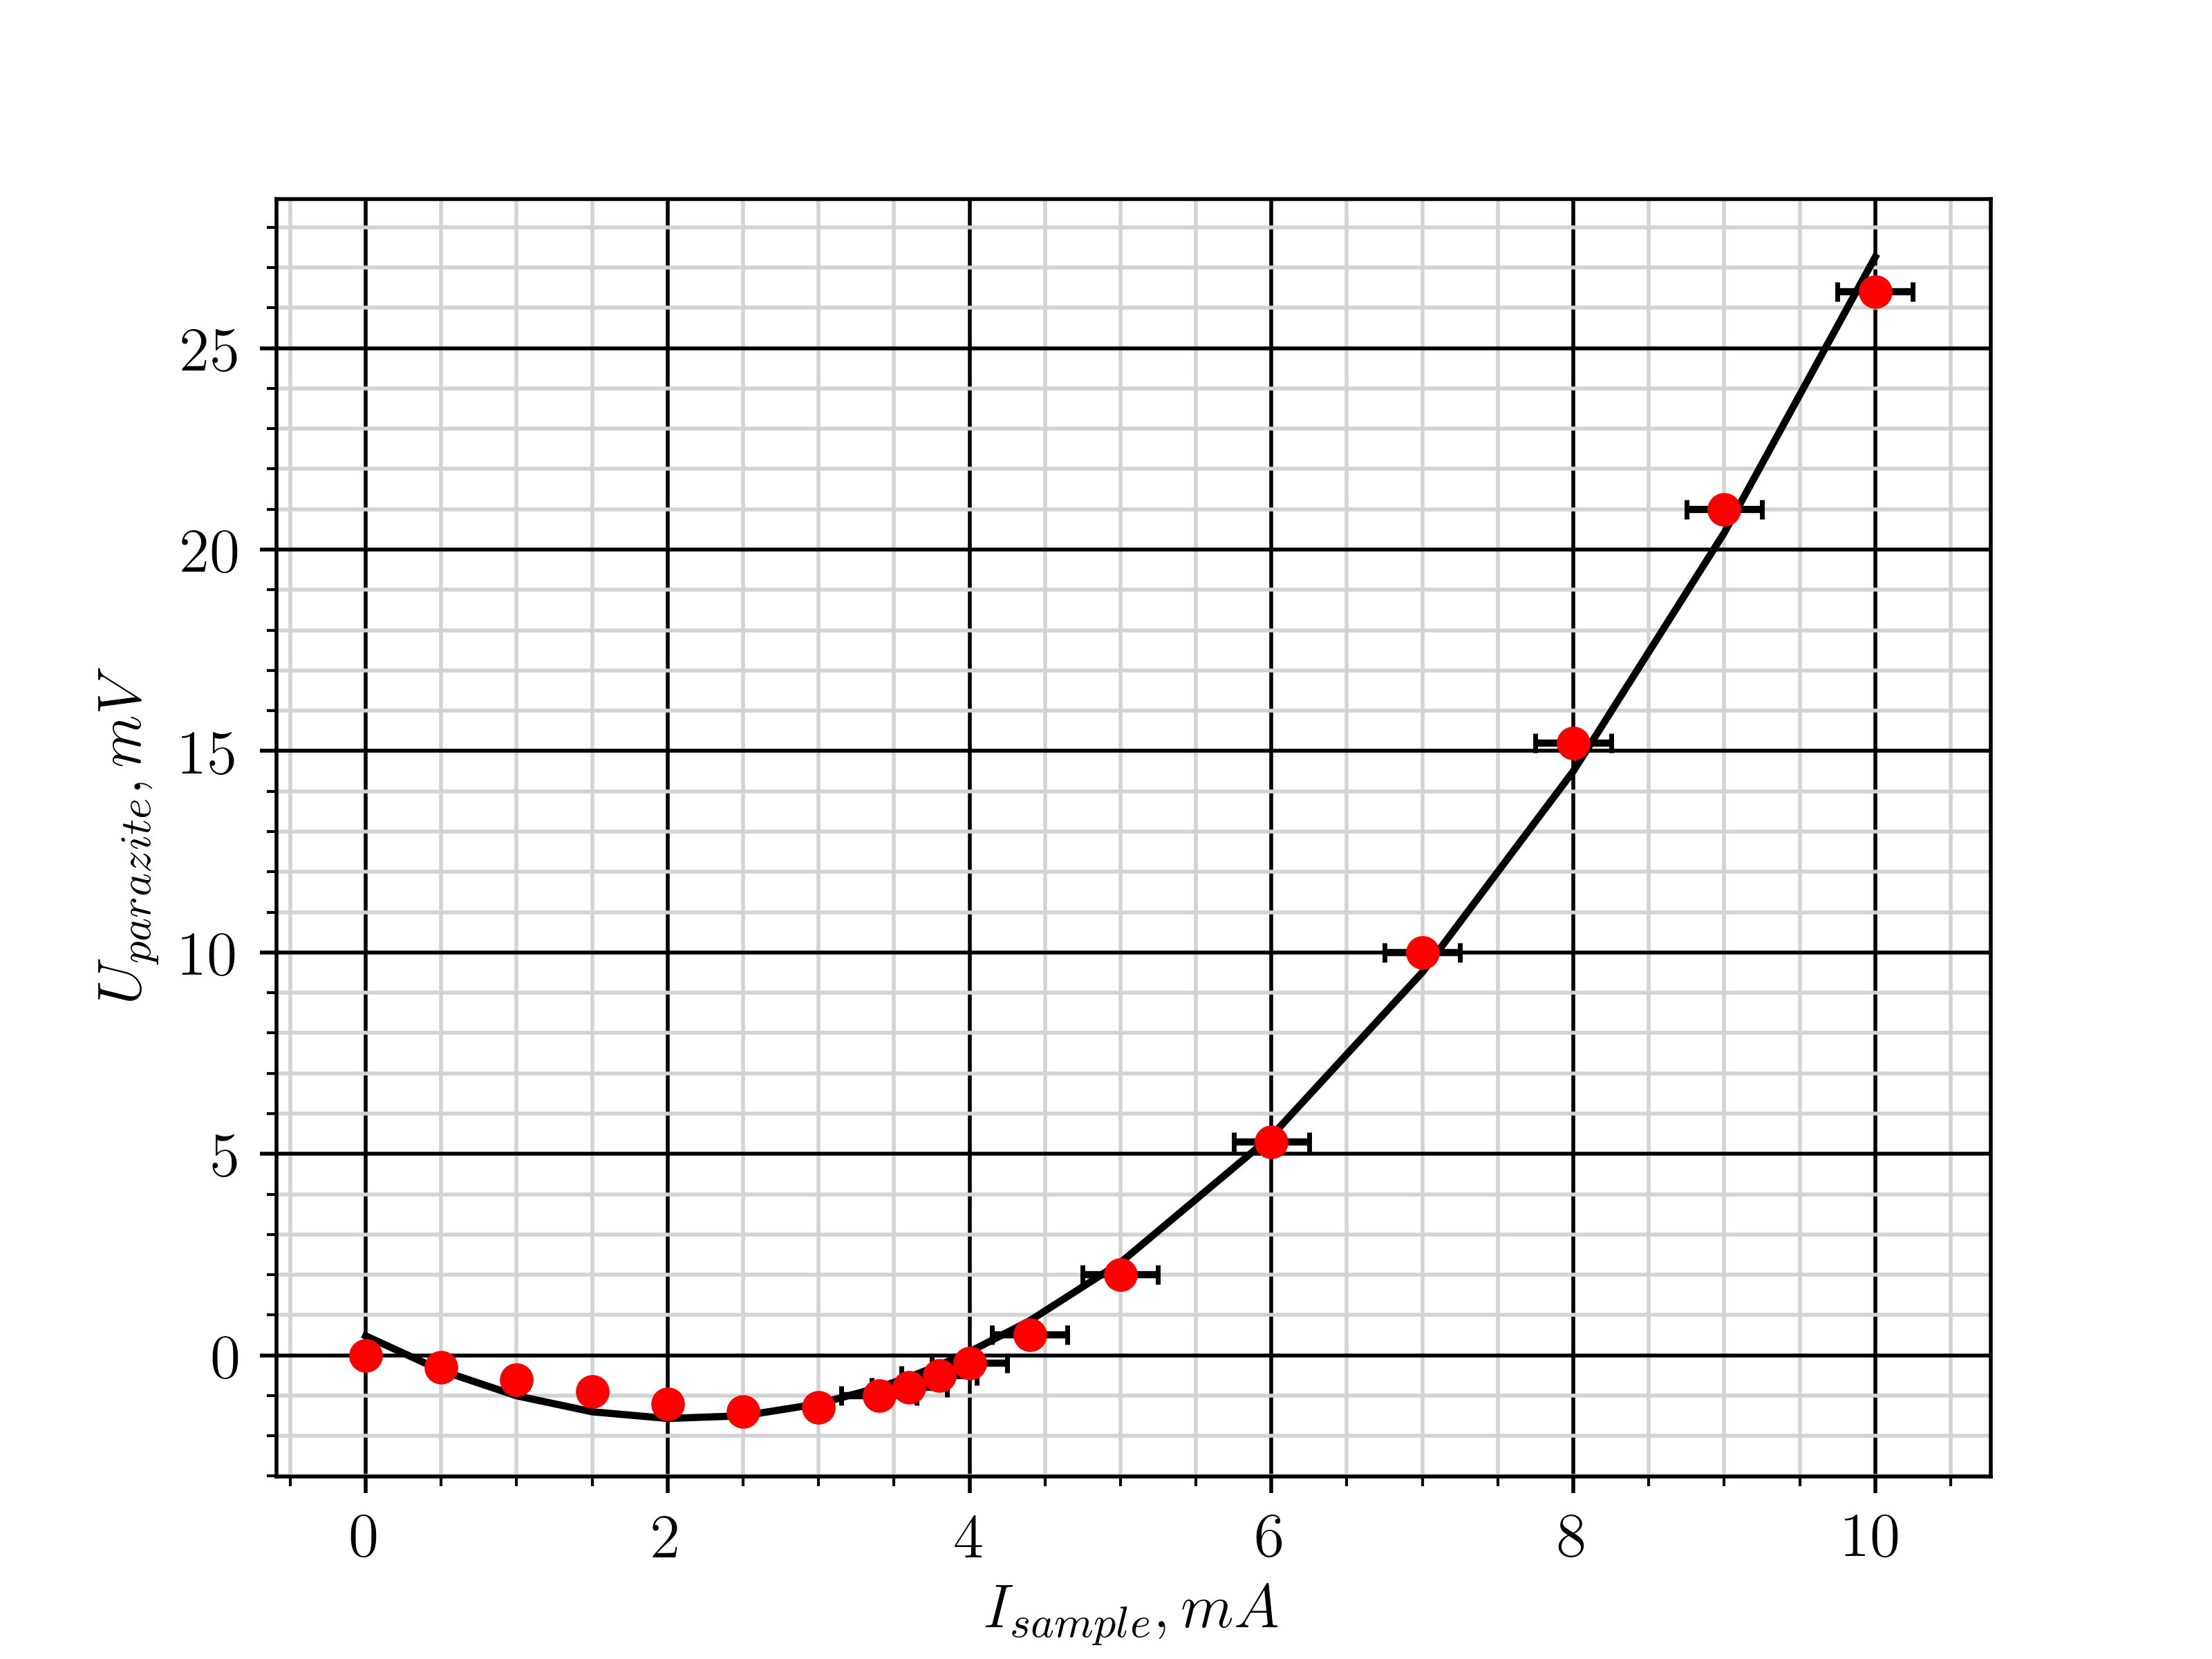
\includegraphics[width = .8\linewidth]{graphs/paraz.png}
		\caption{Паразитное напряжение}
		\label{fig:5.3}
\end{figure}
	
На рис. \ref{fig:5.3} изображена зависимость паразитного напряжения на образце от тока, протекающего через образец.
Кривая паразитного напряжения на контактах снималась при токе в диапазоне $0\ldots10$ мА.(Погрешность тока $\Delta
I_{sample} = I_{\max}\cdot 2.5\% = \pm 0.25 \text{ мА}$, погрешность напряжения $\Delta U = \pm 0.1 mV$)
В последующих экспериментах из снятого напряжения на контактах везде вычитались значения паразитного напряжения.

\subsection*{Определение типа основных носителей в образце}

\begin{figure}[h!]
	\centering
	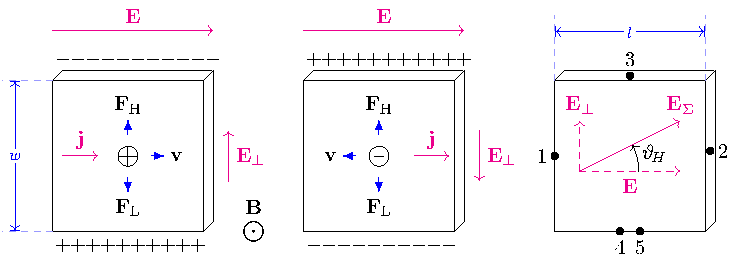
\includegraphics[width=\linewidth]{fig/effect.pdf}
	\caption{Эффект Холла при дырочной и электронной проводимости}
	\label{fig:hall}
\end{figure}

Зная направление магнитного поля и схему включения образца, можно найти тип носителей полупроводника.

Ток течет от контакта 1 к контакту 2, милливольтметр подключен клеммой <<+>> к нижней грани образца (через балансировочную цепь к контактам 4 и 5) и клеммой
<<->> к верхней грани (контакт 3). 

Сила, действующая на заряд в магнитном поле, вызывает разделение зарядов по боковым граням полупроводника, при этом на
гранях возникает разность потенциалов (для дырочного и электронного случая на рис. \ref{fig:hall} показано разделение
зарядов)

Милливольтметр снимал положительное напряжение при данных условиях, и согласно приведенным выше соображениям, носители заряда -- дырки.

\subsection*{Расчёт постоянной Холла и подвижности основных носителей}
Согласно формуле \eqref{eq:2.5}, в линейном приближении можно, зафиксировав одну из переменных (поле магнита или ток), и
снимая зависимость от другой переменной, найти постоянную Холла. Сначала фиксировался ток образца, а потом ток через электромагнит.
\subsection*{Фиксированный ток в образце}
 % зная величину тока или магнитного поля , можно найти  из рисунков \ref{fig:5.5} и \ref{fig:5.6} отношение постоянной Холла к его поперечному размеру.
\begin{figure}[H]
	\centering
	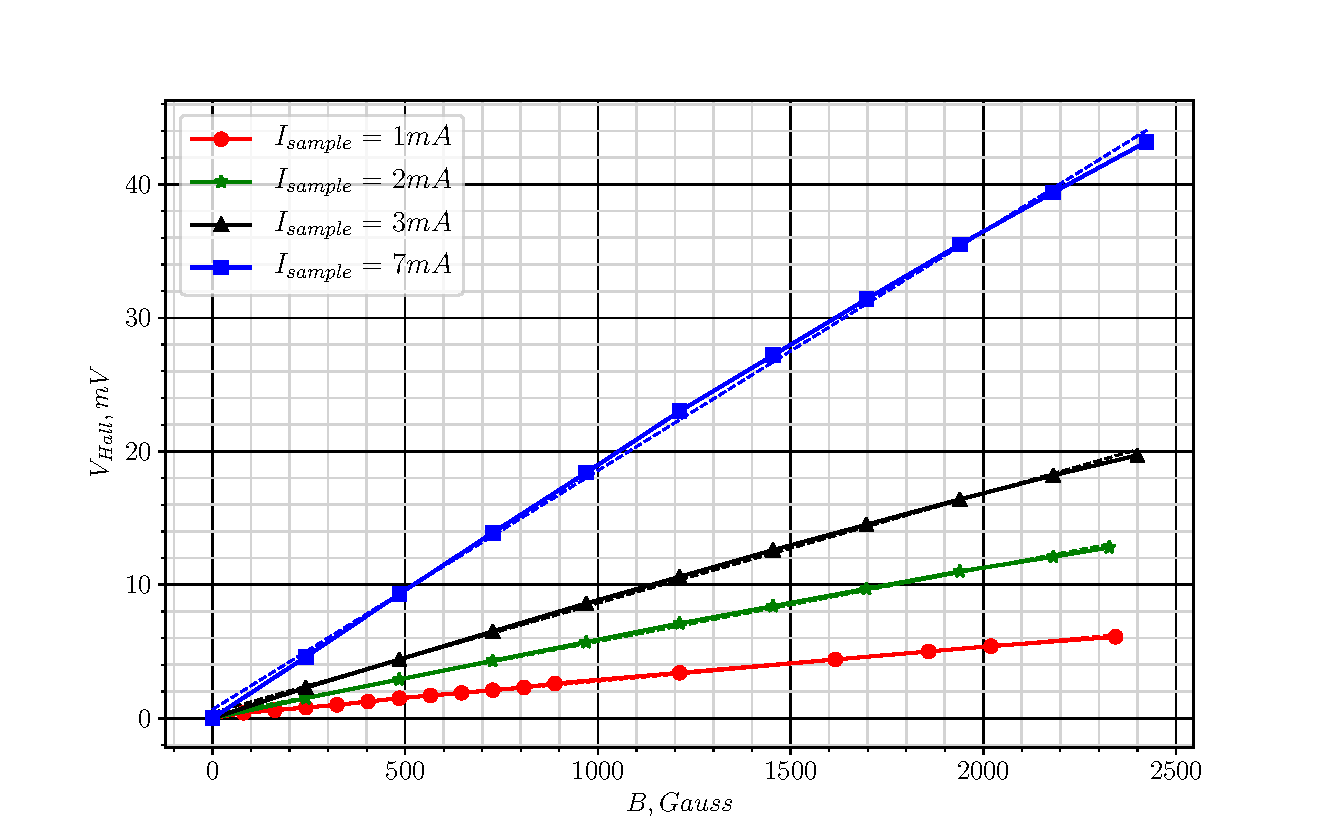
\includegraphics[width = .98\linewidth]{graphs/cc.pdf}
	\caption{Зависимость ЭДС Холла от напряженности магнитного поля при фиксированном значении тока образца(с учётом паразитного напряжения на контактах).}
	\label{fig:5.5}
\end{figure}

В эксперименте фиксировались значения тока образца (от 1 до 7 мА) и при них снимали зависимость напряжения
$V_{Hall}$ от напряженности поля электромагнита. Полученные зависимости построены на графике \ref{fig:5.5}( Погрешности:
$\Delta V_{Hall} = \pm 0.1 \text{ мВ}$, $\Delta B = \pm 808\cdot 0.1\text{ Гс}$, $\Delta I_\text{обр} = I_{\max}\cdot 2.5\% = \pm 0.25  \text{ мА}$ ). 

Для каждого значения тока образца была проведена линейная регрессия, исходя из неё (с учетом коэффициента детерминации $r^2$) и инструментальных
погрешностей были найдены соответствующие значения постоянной Холла:
\begin{gather}
	R_1= (8.52\pm0.3)\cdot10^{-4} \Rdim, 	\quad
R_2= (9.1\pm0.3)\cdot10^{-4} \Rdim,\\
R_{3}= (9.04\pm0.5)\cdot10^{-4} \Rdim, 	\quad
R_7= (8.44\pm0.9)\cdot10^{-4} \Rdim
\end{gather}
\begin{equation}
	\mean{R_{H}} = (8.78\pm0.5)\cdot10^{-4} \Rdim
\end{equation}

\subsection*{Фиксированное поле в образце}
В эксперименте фиксировались значения тока катушки (от 0.25 до 1 А, от 200 до 800 Гс соответственно) и при них снимали
зависимость напряжения $V_{Hall}$ от тока образца.
\begin{figure}[H]
	\centering
	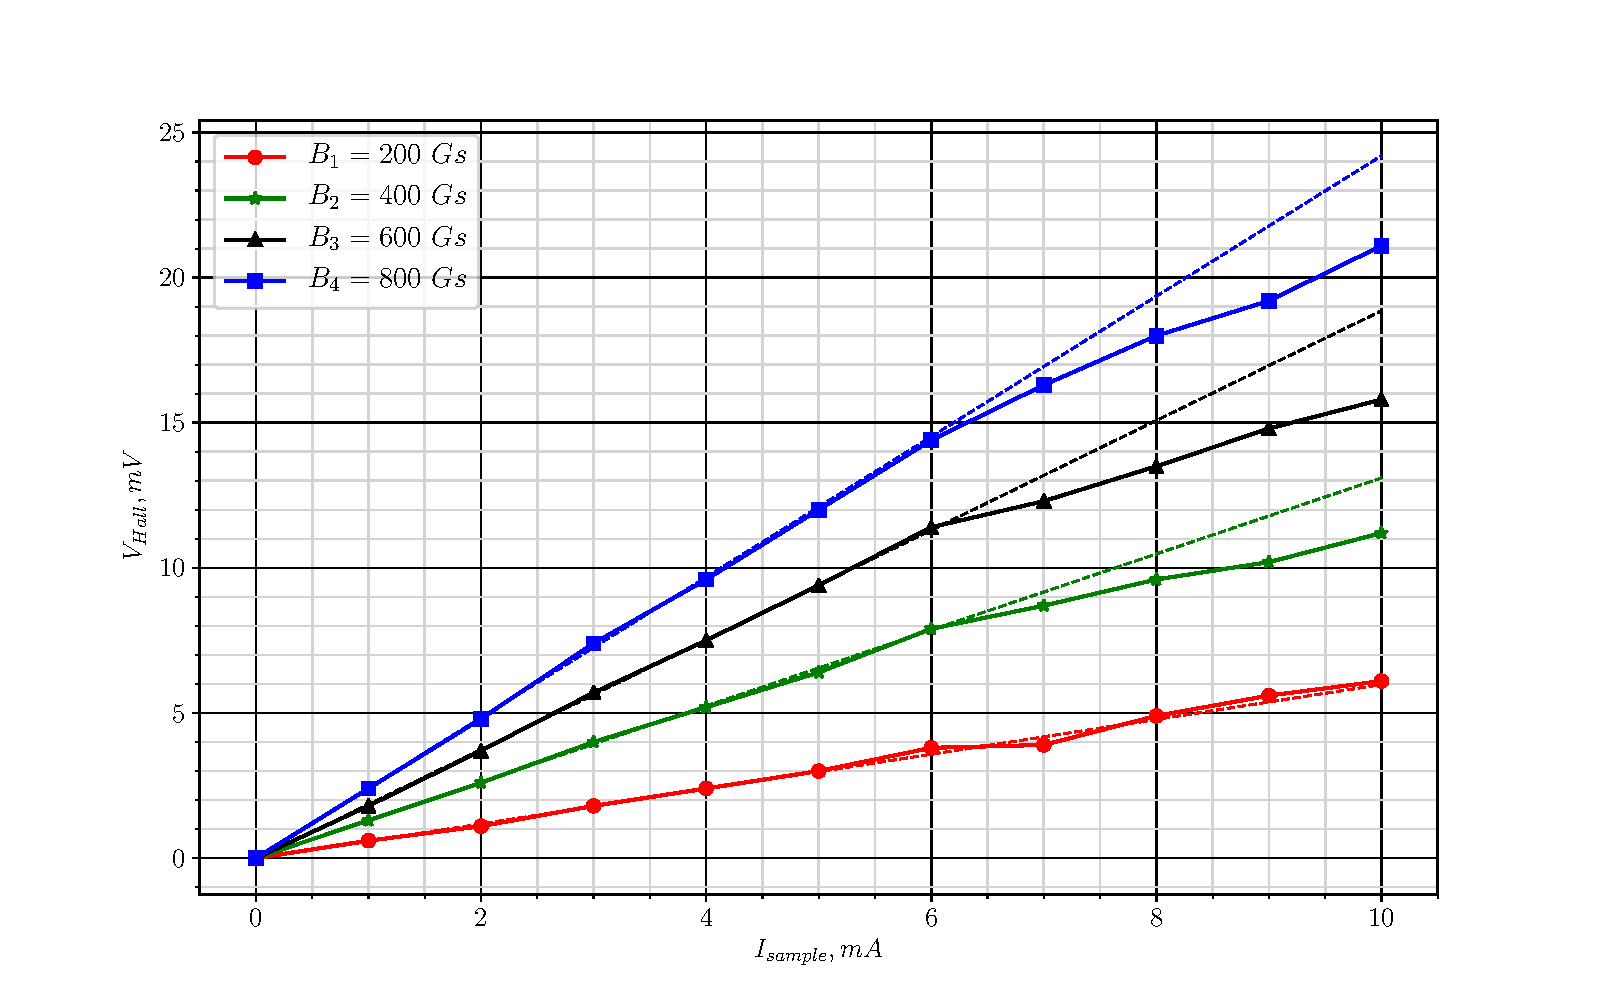
\includegraphics[width = .96\linewidth]{graphs/cf.pdf}
	\caption{Зависимость ЭДС Холла от тока образца при нескольких фиксированных значениях магнитного поля. График построен с учётом паразитного напряжения на контактах.}
	\label{fig:5.6}
\end{figure}

Расчет постоянной Холла аналогичен предыдущему пункту. Отличие в том, что при повышении тока через образец
появляются нелинейные эффекты, и элементарная терия эффекта Холла перестает работать. Поэтому подбор линейной регрессии
осуществлялся таким образом, чтобы прямая наилучшим образом аппроксимировала экспериментальные точки на линейном участке
(см. рис. \ref{fig:5.6}). В результате расчетов получили значения постоянной Холла для каждого значения напряженности:

\begin{gather}
	R_{200}= (9.8\pm0.3)\cdot10^{-4} \Rdim, 	\quad
R_{400}= (10.7\pm0.4)\cdot10^{-4} \Rdim,\\
R_{600}= (10.3\pm0.4)\cdot10^{-4} \Rdim, 	\quad
R_{800}= (9.88\pm0.4)\cdot10^{-4} \Rdim
\end{gather}
\begin{equation}
	\mean{R_{H}} = (10.17\pm0.4)\cdot10^{-4} \Rdim
\end{equation}
\subsection{Обработка результатов}
Из полученных в предыдущих экспериментах значений можем найти среднее значение постоянной Холла:
\begin{equation}
	\mean{R_{H}\hspace{0.1em}}=(9.45\pm0.5)\cdot10^{-4} \Rdim
\end{equation}
Посчитав значение постоянной Холла и удельной проводимости, можно оценить подвижность основных носителей в образце:
\begin{equation}
	\mean{\mu_{\hspace{-0.1em}H}}= \mean{R_{H}\hspace{0.1em}}\cdot \sigma=(3.35\pm0.19)\cdot10^{-2} \,\,\frac{\text{м}^2}{\text{В}\cdot \text{c}}
\end{equation}
Также можно оценить концентрацию основных носителей(дырок):
\begin{equation}
	\mean{p} = \frac{3\pi}{8 R_{H}e} \approx 10^{22}  \text{ м$^{-3}$}	
\end{equation}

\section*{Итоги}
В данной работе был изучен эффект Холла, определен тип носителей заряда исходного образца. 
Определена постоянная Холла, оценена концентрация носителей в образце, подвижность носителей и проводимость образца
\begin{itemize}
	\item $\mean{R\hspace{0.1em}}=(9.45\pm0.4)\cdot10^{-4} \Rdim$
	\item $p\sim 10^{22} \text{ м$^{-3}$}$
	\item $\mean{\mu_{\hspace{-0.1em}H}}= \mean{R\hspace{0.1em}}\cdot \sigma=(3.35\pm0.19)\cdot10^{-2} \,\,\frac{\text{м}^2}{\text{В}\cdot \text{c}}$
	\item $\sigma=34.1\pm0.1 \text{ Ом$^{-1}\cdot$м$^{-1}$}$
\end{itemize}


\end{document}